\documentclass[conference]{IEEEtran}
\usepackage{cite}
\usepackage{amsmath,amssymb,amsfonts}
\usepackage{algorithmic}
\usepackage{graphicx}
\usepackage{textcomp}
\usepackage{xcolor}
\usepackage{hyperref}
\usepackage{float}
\usepackage{booktabs}
\def\BibTeX{{\rm B\kern-.05em{\sc i\kern-.025em b}\kern-.08em T\kern-.1667em\lower.7ex\hbox{E}\kern-.125emX}}
\begin{document}

    \title{Accelerating AI: A Comparative Analysis of GPUs, TPUs, and their Performance}

    \author{\IEEEauthorblockN{Abel Haris Harsono\IEEEauthorrefmark{1},
        Arnav Varshney\IEEEauthorrefmark{2}, Filbert David Tejalaksana\IEEEauthorrefmark{3}}
    \IEEEauthorblockA{\textit{Department of Electrical and Electronic Engineering} \\
    \textit{The University of Hong Kong}\\
    Hong Kong \\
    \{ u3583434\IEEEauthorrefmark{1}, arnav\IEEEauthorrefmark{2}, f1lbert\IEEEauthorrefmark{3} \}@connect.hku.hk}
    }

    \maketitle

    \begin{abstract}
        This document is a model and instructions for \LaTeX.
        This and the IEEEtran.cls file define the components of your paper [title, text, heads, etc.].
        *CRITICAL: Do Not Use Symbols, Special Characters, Footnotes,
        or Math in Paper Title or Abstract.
    \end{abstract}

    \begin{IEEEkeywords}
        component, formatting, style, styling, insert
    \end{IEEEkeywords}


    \section{Introduction}
    \label{sec:introduction}

    Deep learning algorithms, particularly neural networks with millions of parameters, have demonstrated exceptional capabilities in solving complex tasks such as image recognition, speech synthesis, and language translation.
    However, the computational demands of training and deploying these models pose significant challenges for traditional CPUs (Central Processing Units) and even Graphics Processing Units (GPUs).
    To address this issue, specialized hardware accelerators specifically designed for deep learning workloads have gained immense popularity such as Google's Tensor Processing Unit (TPU).

    Google's TPUv4, Nvidia's A100 GPU, and AMD's Radeon VII GPU have emerged as prominent contenders in the market, representing cutting-edge architectures tailored to accelerate deep learning tasks.
    While both platforms aim to deliver high performance, they adopt different approaches to achieve optimal efficiency.
    The TPU is a custom-built application-specific integrated circuit (ASIC) designed by Google, while the A100 leverages the Ampere architecture from Nvidia.

    This paper presents a detailed comparative analysis of Google's TPUv4 and Nvidia's A100, focusing on their architectural characteristics, computational capabilities, memory systems, and power efficiency.
    Furthermore,
    the performance of several accelerators (both GPUs and TPUs)
    is evaluated across computation-intensive operations (CIOs) and a range of deep learning benchmarks.
    A brief discussion on the impact of each platform's design choices on the overall performance and usability is also provided.

    Finally, the paper is concluded with a brief outline on potential avenues for future research in the field of deep learning hardware accelerators.
    The results of this comparative study will aid researchers, developers,
    and practitioners
    in making informed decisions
    when selecting the most appropriate platform for their specific deep learning requirements.
    Furthermore,
    the problems
    revealed in the evaluation results would prove useful in hardware and software design iterations for further optimization.


    \section{Nvidia A100 Tensor Core GPU}
    \label{sec:nvidia-a100-tensor-core-gpu}
    \subsection{Introduction}
\label{subsec:introduction}
Deep neural networks are usually composed of sequential interconnected layers \cite{b3}.
This structure allows for extreme parallelism as computations are broken into smaller chunks, albeit still dependent on its previous layers.
Each layer in a neural network takes in an activation tensor as well as a weight tensor.
An activation tensor represents the output of a single node in the layer, while a weight tensor represents the learning parameters in the network.
The computation between the two tensors involves a mathematical expression similar to matrix multiplications, outputting an activation tensor fed on to the next layer.

\subsection{SM Core}
\label{subsec:sm-core}
The structure of the A100's Streaming Multiprocessor (SM) core works via a 5-step process \cite{b4}.
The A100's memory hierarchy starts with the off-chip DRAM\@ \cite{b5}.
The DRAM provides global access to resources for the SMs.
Data is first loaded from the DRAM into the on-chip L2 cache, acting as a large pool of shared memory accessible by all SMs.
An asynchronous instruction will then be used to partition the data resource for SMEM usage individually and concurrently without blocking the main execution pipeline.
Think of the instruction as an asynchronous implicit duplicate instruction that allows data to be loaded directly from the main memory into a shared memory.
The SMEM connects to the tensor cores via a register file, which acts as a high-speed buffer location, allowing tensor cores to efficiently read and write data to and from the SMEM\@.

\begin{figure}[htbp!]
    \centerline{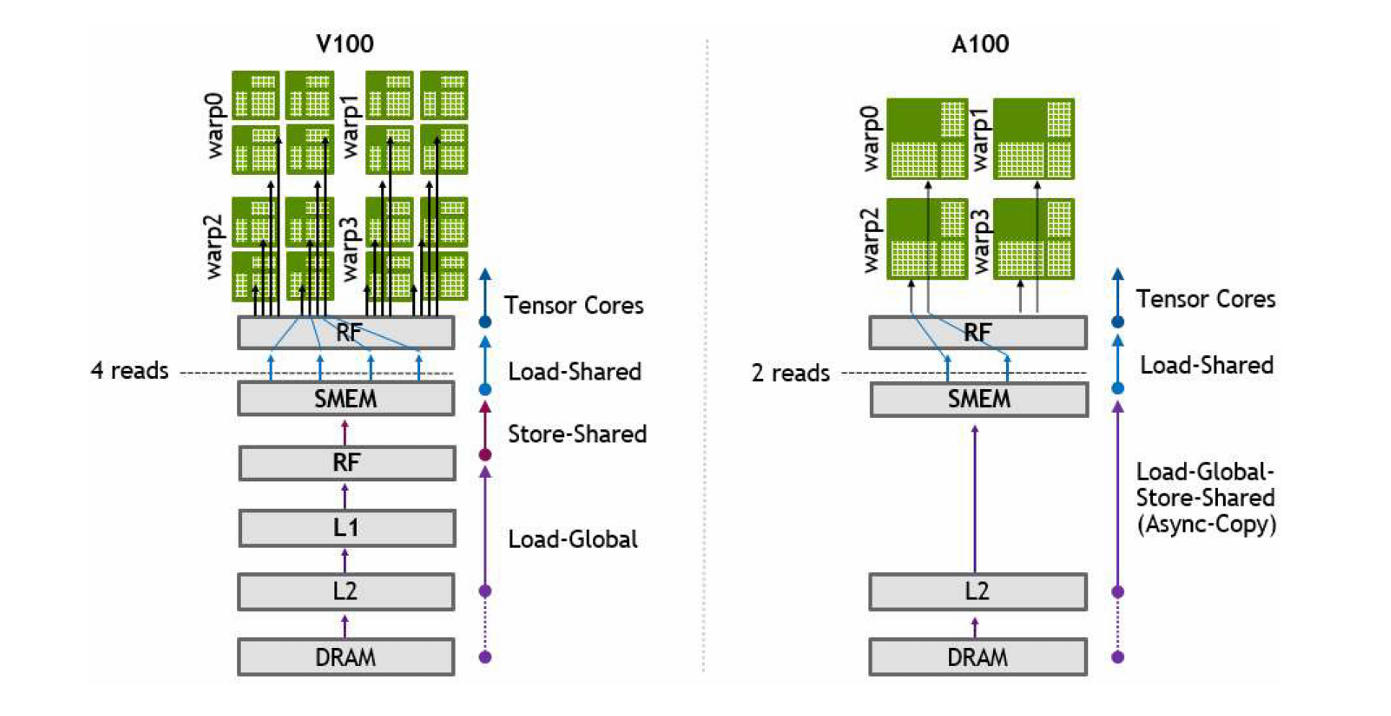
\includegraphics[width=0.5\textwidth]{images/gpu_structure}}
    \caption{V100 vs. A100 structure.}
    \label{fig:v100a100struct}
\end{figure}

To provide context for the specific design of the A100, its predecessor, the V100 can be examined.
The V100 works with a 7-step process.
In the same fashion, data is loaded into an L2 cache from the DRAM, but instead of a direct connection to the SMEM, the V100 requires an additional layer of caching.
By having a dedicated L1 cache per SM, the V100 can make better use of the available memory bandwidth.
Each SM can access its own L1 cache independently, reducing contention and improving overall throughput.
The V100 lacks the asynchronous ``load and store'' instruction in its instruction set; thus it requires an explicit ``write'' instruction to the SMEM to transfer data.

\begin{figure}[htbp!]
    \centerline{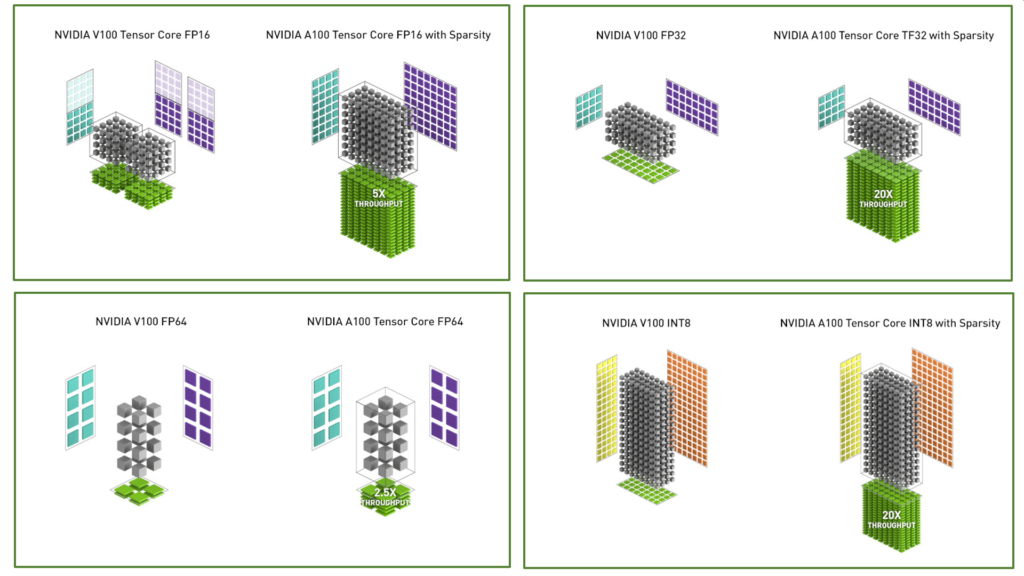
\includegraphics[width=0.5\textwidth]{images/gpu_sparsity}}
    \caption{V100 vs. A100 sparsity.}
    \label{fig:v100a100spars}
\end{figure}

The simplification of the V100 design into the A100 is actually caused by the massive throughput of the tensor core itself.
In both the V100 and A100 designs, the neural network workloads break down each tile into four smaller workable tiles that can be processed in parallel.
A 32-thread warp will then process each of those tiles.
The V100 tensor cores were designed to work with 8-thread granularity, meaning each tensor core operation would process eight threads simultaneously, while the A100 works with 32-thread granularity.
``Fig. \ref{fig:v100a100struct}'' shows the structure of the V100 and A100, while ``Fig. \ref{fig:v100a100spars}'' shows the sparsity of the V100 and A100, comparing the V100’s and A100’s standard operation with multiple data types.
The data types given such as TF32 and TF16 are much more efficient in using tensor-accelerated math than its floating point counterparts, having the same exponent range, albeit less precision.

The 8-thread granularity of the V100's individual network tiles forces it to have a proportionally higher number of load from memory and lower bandwidth in the SMEM, since the 8-thread granularity combined with the fact that data has to move from the L2 cache, to the L1 cache and then to the SMEM, results in higher number of memory access operations per tile.
Reorganizing the A100 to use 32-thread granularity allows it to process a full warp of 32 threads all at once, coupled with improvements in memory access, changed the memory access count from 1 L1 read, 1 SMEM write and 4 SMEM reads into just two SMEM reads per tile.
This reduction in memory access simplifies the data path by relying more on the higher bandwidth SMEM connecting directly without intermediary storage.

\subsection{L2 Cache}
\label{subsec:l2-cache}
An L2 cache in the A100 is a globally shared resource for the SMs.
The A100 divides its L2 cache partitions into two distinct partitions: high-bandwidth access and low latency memory access.
The cache allows for a significant increase in machine learning workloads, with larger datasets and models now being able to be cached and repeatedly hit, contrasting to the V100 requiring slower reading and writing, from and to the HBM2 memory.
The prime enabler of the partition is the L2 Cache Residency Control.
The residency control basically enables a partition of the cache to be used for persistent data access.The A100 employs two key mechanisms to manage persistent accesses to the L2 cache:

\subsubsection{Address-based Persistent Window} Specified address range or “window” will be cached instead of caching a single address and designated to be resident.
Read and write access would be a guaranteed hit in the window.
This method benefits from array-like or consecutive structures such as neural network parameters.

\subsubsection{Per-Memory-Operation Persistent Control} The residency control exposes control over Individual memory accesses to be tagged as persistent by the user, otherwise individual access will not be tagged.
These two persistent access mechanisms work together to optimize the utilization of the L2 cache.
Cache Residency only allows cache tagging when there is ``group access'' to a particular address at a close time, while individual memory access will bypass cache, or can be controlled directly by user to persist.

\subsection{DRAM}
\label{subsec:dram}
The A100 DRAM uses HBM2 memory technology.
The DRAM consists of five of these HBM2 memory stacks, laid vertically and connected to the GPU die via high-speed interconnects.
The tight integration reduces memory latency, power consumption, and its compact stack design aids in the memory having a smaller physical footprint compared to traditional GDDR memory.

\subsection{Closing}
\label{subsec:closing}
The NVIDIA A100 GPU marks a significant advancement in GPU architecture, leveraging innovative hardware designs.
From streamlining its preceding 7-step process of the SM core to a 5-step process, to including compression and residency algorithms to the cache, and introducing asynchronous partitioning instruction to enable direct data transfer to high-bandwidth SMEM\@.


    \section{Tensor Processing Unit}
    \label{sec:tensor-processing-unit}
    \subsection{Introduction}
\label{subsec:introduction2}
A TPU is similar in nature to a GPU or even that of a CPU: they are the ones who are performing the computations within a system.
What distinguish the TPU from the rest is how and what kind of computations are being carried out.
While GPUs and CPUs are considered general purpose, TPUs are an application-specific integrated circuit (ASIC).
Developed by Google, they are built to accelerate performance of Machine Learning (ML) related applications, particularly their linear algebraic processes that involve matrices.
This is also reflected by the hardware incorporated into them.
As a consequence, however, they cannot do much else, at least not efficiently.
The Tensor Processing Unit (TPU) has currently evolved to its fifth version.
However, for the purposes of this work, only TPUv4 will be discussed, highlighting its important features.

\subsection{Structure}
\label{subsec:structure}
There are 2 main components to a TPU chip: High Bandwidth Memory (HBM) and the Tensor Cores (TC).
The HBM is an on-chip memory allowing for larger models and bigger batch sizes to utilize.
The TCs on the other hand consist of many multiply-accumulators; the special hardware that allows for an increase in speed for the matrix-related operations.
These multiply-accumulators are all arranged in an array-like structure, called the systolic array structure, within the chip.

Google’s TPU machine consists of thousands of these TPU chips (as of TPUv4, there are 4096 chips placed inside).
Within the machine itself, the chips are arranged physically as separate 4 x 4 x 4 cube but the inner networking between the chips, their logical connection, is more flexible and can be defined by the user.
For instance, by default, the connections would resemble a torus.
Furthermore, within this system, a CPU is also in use.
With TPUv4, there is one CPU for every 4 TPU chips resulting in around 1000 CPUs in total.

The TPU works by first loading parameters from the HBM into individual multiply-accumulators and then feed the data/input/activation to one row/column of the array-like architecture.
The results of one computation feed the next one, and so on, similar to how a ripple-carry adder works.

\subsection{TPUv4}
\label{subsec:tpuv4}
The main improvements introduced by TPUv4 mainly handle around the subject of scale and reliability using Google's very own advancement in optical switches.
Additionally, just as any other kind of iteration, the TPUv4 also improves certain aspects of the system.
For example, the storage of embeddings is dealt by introducing appropriate hardware architectures and a way that allows for a better compatibility between hardware and the model was also introduced.

\subsubsection{Reconfigurable Optical Switches}
The TPUv4 is equipped with 4096 TPU chips.
While this quantity might not appear significant, it becomes noteworthy when contrasted with the TPUv3, which only had 1024 chips.
The sheer size of the TPUv4 renders electrical switches useless due to ``electrical interconnect'' limitations.
To solve this, optical switches were used.
In particular, Google's Palomar Optically Configurable Switches (OCS).
They are based on Micro-Electro-Mechanical Systems that can send light both ways in a fiber by employing what is called a ``circulator''.

\begin{figure}[htbp!]
    \centerline{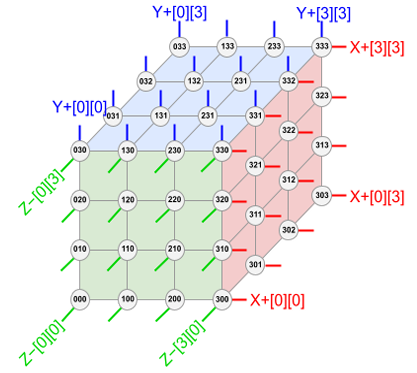
\includegraphics[width=0.2\textwidth]{images/tpu_cube}
    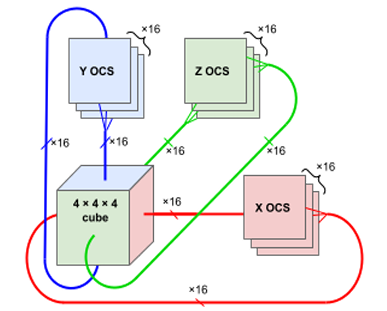
\includegraphics[width=0.2\textwidth]{images/tpu_connectivity}}
    \caption{OCS Architecture.}
    \label{fig:ocsarch}
\end{figure}

``Fig.\ref{fig:ocsarch}'' illustrates how the OCSs are connected.
This cube, a 4 x 4 x 4, is part of the TPU machine that consists of many TPU chips that must be connected to the OCS\@.
A cubic arrangement of 64 chips is considered due to nicer bisection bandwidth and for convenience in storage.
To connect, each side and its corresponding opposite side of the cube are connected to the same OCS\@.
In total, for TPUv4, there are typically 3 * 16 = 48 OCSs for a single machine.

The OCS brings a multitude of benefits.
The first being availability and deployment benefits.
Being flexible and having better performance allows TPUv4 to still provide good services, even when some chips of the system may not be available.
And because the OCSs bring some sort of independence to the system (particularly, it made each rack of the machine more independent), not all chips are needed to ensure operability.

Second, the most obvious one, configurability.
The OCS greatly simplifies scheduling and networking within the system due to its great switching speed.
For instance, it no longer has to search for many contiguous chips during scheduling as required by the previous version and the OCS. It allows modularity between users (the whole system can cater to multiple users) which enhances security.
Finally, the logical connection can be easily reconfigured to one's topological needs, typically to exploit different kind of parallelisms (i.e., Data, Model, and Pipeline parallelism), as ``rewiring'' the system mostly involves reprogramming the routes of the OCS\@.

\subsubsection{SparseCore}
Like any other computers dealing with ML, this one is for dealing with embedding.
In particular, where to store the lookup tables from the embedding process.
The main problem here is that the lookup operations will cause a bottleneck for the chips due to memory accesses, inter-chip communication, etc.
As they are more suited for dense arithmetic operation.

In this context, there were two possible solutions: either put it in the CPU or put it in the tensor cores themselves.
The CPU approach would introduce a bottleneck during the next iterations by Amdahl’s law; in comparison, there is a 4:1 TPUv4 to host CPU ratio.
On the other hand, putting it in the TC would be suboptimal due to them being optimized for dense operations.
A way out of this is to use both the HBM and the dedicated Inter-Core Interconnect (ICI) network which are embedded in the chips.
With these in mind, comes SparseCore (SC).
It is an additional hardware put in the machine for dealing with embedding training.
SC uses the HBM and a dedicated ICI network while operating in a sea of cores configuration creating a flat, globally addressable memory space.

Although SC seems to only handle storage of embeddings, it actually behaves almost as a whole package to deal with sparse data related operations.
Mainly, it consists of 16 compute tiles and 5 Cross-Channel inputs for performing preprocessing of the sparse input.
Each compute tile consists of a fetch unit, Single Instruction Multiple Data (SIMD) Vector Processing Unit, the Sparse Vector Memory for storing data read from the fetch unit, and the flush unit utilized during backward propagation.

\subsubsection{Platform-Aware Neural Architecture Search}
Platform-Aware Neural Architecture Search or PA-NAS has a goal to configure both the ML model and the TPU topology to benefit from each other as much as possible.
In particular, with the mention of SC, a model in the TPU might need to use both SC and TC efficiently.
PA-NAS optimizes operations related to this to achieve ``pareto-optimal performance and quality''.


    \section{Performance Evaluation}
    \label{sec:performance-evaluation}
    \subsection{Introduction}
\label{subsec:introduction3}




    \section{Contribution Statement}
    \label{sec:contribution-statement}
    \begin{itemize}
        \item Abel Haris Harsono: 33.3\%
        \item Arnav Varshney: 33.3\%
        \item Filbert David Tejalaksana: 33.3\%
    \end{itemize}

    \label{itm:refs}
    \begin{thebibliography}{00}
    \bibitem{b1} X. Mei, Q. Wang, and X. Chu, ``A Survey and Measurement Study of GPU DVFS on Energy Conservation.'' arXiv, Oct. 06, 2016. doi: \href{https://doi.org/10.48550/arXiv.1610.01784}{10.48550/arXiv.1610.01784}. New York, NY, USA: Association for Computing Machinery, May 2017, pp. 1–11. doi: \href{https://doi.org/10.1145/3077839.3077855}{10.1145/3077839.3077855}.
    \bibitem{b2} V. Chau, X. Chu, H. Liu, and Y.-W. Leung, “Energy Efficient Job Scheduling with DVFS for CPU-GPU Heterogeneous Systems,” in \textit{Proceedings of the Eighth International Conference on Future Energy Systems}, in e-Energy ’17.
    \bibitem{b3} J. Choquette, W. Gandhi, O. Giroux, N. Stam, and R. Krashinsky, “NVIDIA A100 Tensor Core GPU: Performance and Innovation,” IEEE Micro, vol. 41, no. 2, pp. 29–35, Mar. 2021, doi: \href{https://doi.org/10.1109/mm.2021.3061394}{https://doi.org/10.1109/mm.2021.3061394}.
    \bibitem{b4} “NVIDIA Tesla P100.” Available: \href{https://images.nvidia.com/content/pdf/tesla/whitepaper/pascal-architecture whitepaper.pdf}
    \bibitem{b5} R. Krashinsky, O. Giroux, S. Jones, N. Stam, and S. Ramaswamy, “NVIDIA Ampere Architecture In-Depth,” NVIDIA Technical Blog, May 14, 2020. \href{https://developer.nvidia.com/blog/nvidia-ampere-architecture-in-depth/}{https://doi.org/10.1109/mm.2021.3061394}
    \bibitem{b6} “Introduction to cloud TPU  |  Google Cloud,” Google, \href{https://cloud.google.com/tpu/docs/intro-to-tpu} (accessed Apr. 7, 2024). 
    \bibitem{b7} N. P. Jouppi et al., TPU v4: An Optically Reconfigurable Supercomputer for Machine Learning with Hardware Support for Embeddings. 2023.
\end{thebibliography}


\end{document}
